%%
%% This is file `example/ch_intro.tex',
%% generated with the docstrip utility.
%%
%% The original source files were:
%%
%% install/buptgraduatethesis.dtx  (with options: `ch-intro')
%% 
%% This file is a part of the example of BUPTGraduateThesis.
%% 

\chapter{绪论}
\section{研究背景及其意义}

1. 段路由研究背景

\gls*{SDN} \cite{OPENFLOW, SDN} 场景下,控制器作为网络设备的集中管控面可以获得网络全局信息,但是网络流量全部依靠软件定义网络机制进行调控,就会缺少一些时效性。例如 \gls*{MPLS} 依旧是当前业界最常用的流量工程调度技术之一,其使用的初衷是使用标签替代交换机IP地址以进行快速转发, \gls*{MPLS} \cite{MPLS} 技术按照网络拓扑用控制需求驱动而非更传统的流量驱动,这样就更加优化了流量工程的工作原理。存储资源稀缺 \cite{TCAMMPLS, TCAMSDN} 对标签进行匹配并分配出端口的操作可以不上送CPU就能够完成,因此降低了交换机对报文的处理查表时延和查表复杂度,提高了转发效率。但是在标签分发上需要 \gls*{LDP} 来分配标签,在标签通告上也需要 \gls*{IGP} 或 \gls*{OSPF} 协议进行辅助。除此以外, \gls*{MPLS} 在工作时,每个下一跳都是确定的,即网络中需要有一条隧道完整地预留给某一个策略下的流量 \cite{MPLS} ,这就需要一些对IP网络资源进行协调整合的协议来完成,常用的就是 \gls*{RSVP} \cite{RSVP} 和为了 \gls*{MPLS} 建立标签交换路径而扩展补充出来的 \gls*{RSVP-TE} 。IP网络终端运行的应用程序可以基于资源预留机制向其他节点表明终端所要接收的数据包流的性质(如带宽,抖动,最大突发量等),可以使网络边缘用于计算 \gls*{MPLS} 路径的装置依照数据包流需求进行流量转发路径分配。但是当前的 \gls*{MPLS} 部署方式存在一些弊端:一是 \gls*{RSVP-TE} 的操作开销通常很高;二是IP网络原本可以使用 \gls*{ECMP} 做到原生的负载均衡,但 \gls*{MPLS} 作为显式源路由,将路由路径的标签全部封装在报文头,使得每一跳之间无法进行IP网络原生的多路径负载均衡,容灾和自愈能力较差。

\gls*{SR} \cite*{SRARK} 提供了一种新的流量调度思想,不同于源路由规划好每一跳的路径,段路由只在若干跳的范围规划一个目的段标签,使得段路由报文头的段列表只用很少的段标签就可以指导网络流量转发,这可以看作是软件定义网络控制器对网络流量的处理模式进行编程,段路由的段列表就相当于编程的代码,由此达到对网络数据包进行操作的网络编程目的。目前,产业界已经将段路由广泛应用于监控、流量工程、故障恢复、集中控制架构、路径编码、网络编程、性能评估等诸多领域 \cite{SRSURVEYS}。例如使用 \gls*{SRv6} 支持 IPv6 骨干网和数据中心中的流量工程、服务功能链和虚拟专用网络等服务 \cite{SRUSAGE1, SRUSAGE2};将段路由和带内网络遥测有机结合以实现具有高效和自适应监控优势的新型网络 \cite{SRUSAGE3};运营商网络也在研究如何逐步将段路由增量部署到现有IP网络中 \cite{SRBANDWIDTH7}。

但是针对某一段路由策略的段列表计算需要具有全局视角的段路由控制平面 \cite{SRARK} 来决定,可以通过操作员进行配置,也可以在软件定义网络场景下由控制器进行计算分配。目前常用的标签栈计算方式都是基于带宽的 \cite{SIDLENGTHPROVE, SIDLENGTHANALYSIS, SRQOE, SRMULTIPATH, SRLABELSTACK, SRNODETE, SRBANDWIDTH1, SRBANDWIDTH2, SRBANDWIDTH3, SRBANDWIDTH4, SRBANDWIDTH5, DEFO, SRBANDWIDTH6, SRBANDWIDTH7, SRBANDWIDTH8, SRBANDWIDTH9, SRBANDWIDTH11, SRBANDWIDTH12},而在业务对时延越来敏感的大环境下,就需要考虑使用时延作为指导段列表生成的因素,即在以段路由流量工程为服务质量保障技术代表的网络层对时延进行一定程度的保障。因此本文将分别基于集中式控制和分布式控制对具有时延保障效果的段路由航点列表生成算法进行研究讨论。

2. 时延研究背景

近年来学术界和产业界也在越来越多得关注时延保障的问题,其内在的驱动力主要是时延敏感的业务正在蓬勃发展。随着线上办公、线上会议的普及;元宇宙概念的兴起带来增强现实/虚拟现实/实时视频等技术进一步发展;以及物联网车联网概念下对时延苛刻的要求,越来越多的高 \gls*{SLA} 业务对时延的要求明显增强。因此有必要在网络 \gls*{OSI} 模型中的各个层级对时延保障展开探索。

网络中的时延主要分为节点处理时延(Nodal Processing Delay)、传播时延(Propagation)、传输时延(Transmission Delay)、排队时延(Queuing Delay)。而将上述这些种类的时延全部累加起来就得到通信节点间总时延(Total Nodal Delay)。实际上节点处理时延往往是微秒级别可以忽略不计;传播时延由光信号在光纤中传播产生,本身引起的时延很小且是客观存在无法进一步优化的时延;传输时延指的是在队列中,当分组在链路上等待传输时发生的时延;至于一个特定分组的排队时延则取决于先于本分组到达的、正在排队等待向链路传输的分组的数量。如果该排队队列是空的,即当前没有其他分组在等待传输,那么该分组的排队时延为零,可以立刻得到服务。另一种情况,如果流量很大,并且许多其他分组也在等待传输,那么该分组的排队时延将很大。到达组的分组数量是到达该队列的流量强度和性质的函数。实际的排队时延通常在毫秒到微秒级。

为了优化排队时延,数据链路层上 \gls*{TSN} 技术正在引起很多研究人员的关注。时延敏感网络旨在保证时延敏感业务流量的服务质量,实现低时延、低抖动和零丢包率的高可用网络。其主要的实现方式就是限制发送端的发送功率,从物理层面上压制可能出现的突发流量。在发送功率的确定上需要用排队论、博弈论的思想最终确定一个合适的信息发送功率,并对发送信号进行整形,从发送源头上规避可能出现的排队问题,最终使得业务流量实现超低时延和零丢包,在时延角度看来实际上就是使得排队时延降为零,使得网络中只存在客观的处理时延,而这种时延是可预期可计算的。

传输层由于有 \gls*{TCP} 这种建立端到端链接的协议,对时延更为关注,也更适合在拥塞控制算法中使用时延数据来调整发送窗口,例如在Swift \cite{SWIFT} 中,通过使用 \gls*{AIMD} 的方式来实现端到端的延迟控制,并在极端拥塞的情况下调整步调,通过精确的 \gls*{RTT} 测量并仔细考虑延迟目标。又如 \gls*{HPCC} \cite{HPCC} 利用 \gls*{INT} 来获取精确的链路负载信息并精确控制流量。通过解决拥塞期间延迟的带内遥测信息和对带内遥测信息的过度反应等难题,使得高精度拥塞控制可以迅速收敛以利用空闲带宽,同时避免拥塞,并且可以保持接近零的网络内队列以实现超低延迟。

3. 段路由对时延支持的研究意义

在网络各个层面都开始尝试保障时延的情况下,网络层因为其尽全力交付的特性而难以在端到端时延上作出保证,通常和业务相关的需求都由传输层协议完成。网络层的研究方向里只有流量调度可以为服务质量提供一些保障,而段路由正是流量调度的一种新型方法,由于其灵活性已经被网络设备商广泛支持,也被网络运营商广泛使用,最新的Linux \cite{LINUXSRv6} 内核协议栈也开始支持段路由,因此探索段路由对时延的保障是有一定研究成果支持的。

流量调度中的服务质量需求是多种多样的,目前比较常见的有最小化网络能耗、优化拥塞和最小化被拒绝请求的数量,可见最小化流量时延是一个研究还比较缺乏的领域,因此本文将最小化流量时延或保障时延需求作为流量工程优化的目的,以段路由为主要实现方式进行段路由航点列表算法设计,这对充实在各个 \gls*{OSI} 网络分层中对时延需求进行保障具有一定意义。

\section{课题来源}
本课题研究主要来源于以下项目的支持:

1)国家重点研发计划:支持高级语言编程的SDN控制系统研究(2020YFB1804603);

2)国家重点实验室课题:基于软件定义的天地一体化网络架构(NST20200104)。

\section{国内外研究现状}

本节将简要回顾在传统IP网络(IP-TE, OSPF-TE)、完全部署段路由的网络(SR-TE)和部分部署段路由的网络(混合SR-TE)中使用域间/域内流量调度算法的相关研究以及域间/域内流量调度算法的应用机制。

在传统的IP网络中,每条链路都被分配了一个权重(即链路成本),不同的链路权重设置会导致不同的转发路径。 \gls*{MCF} 问题是一个经典的优化问题,网络工程流量调度方案的计算就是一种 \gls*{MCF} 问题。由于 \gls*{MCF} 问题的复杂性,研究如何在路由优化和流量工程中应用 \gls*{ML} 成为新趋势 \cite{MLALNET} 。机器学习算法可以从过去的网络状态中学习流量发生规律,并为未来的网络状态生成合适的路由配置。与启发式算法相比,机器学习具有更具适应性的视角,而不是依赖于人为确定的启发式方法。 \gls*{SL} 和 \gls*{RL} 是已经应用于流量工程的机器学习的两个分支。监督学习必须从标记的训练数据中学习,这在流量工程领域很难获得。但是,强化学习是从网络环境中学习,而不是通过动作和奖励与网络迭代交互,而不是预先收集的训练数据,因此更适合流量工程。有一些研究人员比较了两种机器学习方法 \cite{MLALNET} :一是使用监督学习来预测即将到来的流量矩阵并根据预测的流量矩阵来优化路由;二是使用强化学习学习从历史流量矩阵到路由配置的较好的映射。他们的工作表明,强化学习在路由优化方面比监督学习更有前景。研究 \cite{MLSR2} 使用 \gls*{DRL} 和 \gls*{DDPG} \cite{MLSR3} 仅通过设置IP网络中的链路权重,就可以一定程度上优化最小化网络时延。有研究 \cite{MLSR1} 则是提出了一种基于深度确定性策略梯度的改进算法,并使用它来决定预定义转发路径上的分流比,而无需指定网络场景。这些研究仅适用于将机器学习尤其是强化学习应用于具有基本决策变量和奖励获取容易的网络场景中。

除了使用机器学习优化流量工程的计算结果,段路由节点与非段路由节点如何共存保障网络架构平滑过渡也是一个常见的研究重点。段路由网络中的一个数据包依次通过一系列段路由,段路由列表(Segment list, SL)由入口路由器确定并封装在数据包头中。段列表中的段数称为 \gls*{SLD} 。目前对段路由流量工程的研究主要可以分为两大类:一是建立段路由的网络模型;二是只关注段路由的路径编码问题。在考虑段路由的情况下构建模型时,一些研究利用了适用于大规模网络的启发式方法。哈特等人 \cite{DEFO} 提出了一个集中式优化器DEFO,它将以北向接口语言表达的高级目标转换为兼容的网络配置。他们使用本地搜索来搜索最合适的段路由航点列表。另外有论文作者专注于段路由网络中转发路径的快速重新路由 \cite{SRFRR1, SRFRR2} 。他们使用预处理、移动预过滤和累积树来加速本地搜索。仍有许多研究 \cite{SRBANDWIDTH8} 使用 \gls*{LP} 解决段路由流量工程问题。这些研究将问题形成为线性规划公式,并使用线性规划求解器进行求解。有研究 \cite{SRBANDWIDTH7} 提出了一种没有使用等价多路径路由的路由流量工程算法。在研究段标签长度时,有作者提出了一种2-段路由 \cite{2SR} 的方法,该方法将每个流的最大段路由列表深度限制为2,并确定离线和在线情况下段路由的最佳参数。在该研究中,作者分析了真实世界的流量并扩展了2-段路由公式以最小化非最短路径隧道的数量。他们还评估了3-段路由和4-段路由的流量工程能力,并表明它们非常耗时,因此较长的段路由深度是不值得提倡的。有研究 \cite{SRBANDWIDTH10} 人员研究了基于软件定义网络的广域网中的段路由流量工程,并证明了一般的段路由策略生成问题是一个NP-hard问题。

段路由的路径编码问题则是旨在将预先计算的流量工程路径编码为一组段列表,同时最小化段列表的大小。现有研究仅考虑全段路由节点网络中的路径编码问题。一些研究将路径分解为几个子路径并分别对它们进行编码 \cite{SRXXXX1, SRXXXX2, SRXXXX3} ,还有一些研究者用辅助图表示转发路径并解决其上的线性规划问题 \cite{SRXXXX4, SRXXXX5} 。

目前,基于混合段路由网络的流量工程还处于起步阶段,相关工作很少。有研究 \cite{SRXXXX6} 提出了一种在考虑流量工程的同时将段路由增量部署到运营商网络的策略。作者假设支持段路由功能的节点构成 \gls*{SRD} ,这限制了入口段路由节点和出口段路由节点之间路径上的所有节点都必须支持段路由。分段路由域的部署方式适用于 \gls*{SR-MPLS} 。但是由于 \gls*{SR-MPLS} 的段路由的特性,不能使用段路由节点段跨不同分段路由域路由流,否则数据包将被非段路由节点丢弃。并且每个分段路由域必须至少有两个段路由节点才能在其内部使用段路由节点。因此,虽然可以通过设置分段路由域数量和段路由数量相等来获得分散部署的IP和段路由共存的混合网络,但它不能使用段路由节点段,所以它不能很好地运作。另外有研究 \cite{SRXXXX7} 采用默认的开放最短路径优先协议链路权重并使用混合整数线性规划(Mixed-integer linear programming, MILP)优化框架来确定最佳分段路由域构成和流量路径。但是,默认链路权重通常设置为与链路容量成反比的现象可能不适用于段路由。由于分段路由域限制和链路权重设置不当,需要50\%以上的节点升级为段路由节点,才能获得与全段路由网络相当的最大链路利用率。以上这些工作的主要特点如下:第一它们只在混合段路由网络中优化具有段路由能力的节点的流量路径和位置,而链路权重是固定不变的;第二是所有网络节点都基于完全部署的段路由网络或混合段路由网络,其中段路由节点部署为分段路由域。这些工作为解决网络过渡阶段混合部署的问题提供了思路。

\section{论文主要结构}

本论文将从段路由的时延保障节点选择,以及基于段路由协议标签列表的时延保障方案的研究点展开,各部分研究内容关系如图1-1所示。

\begin{figure}[htbp]
\setlength{\abovecaptionskip}{15pt plus 3pt minus 2pt}
\centerline{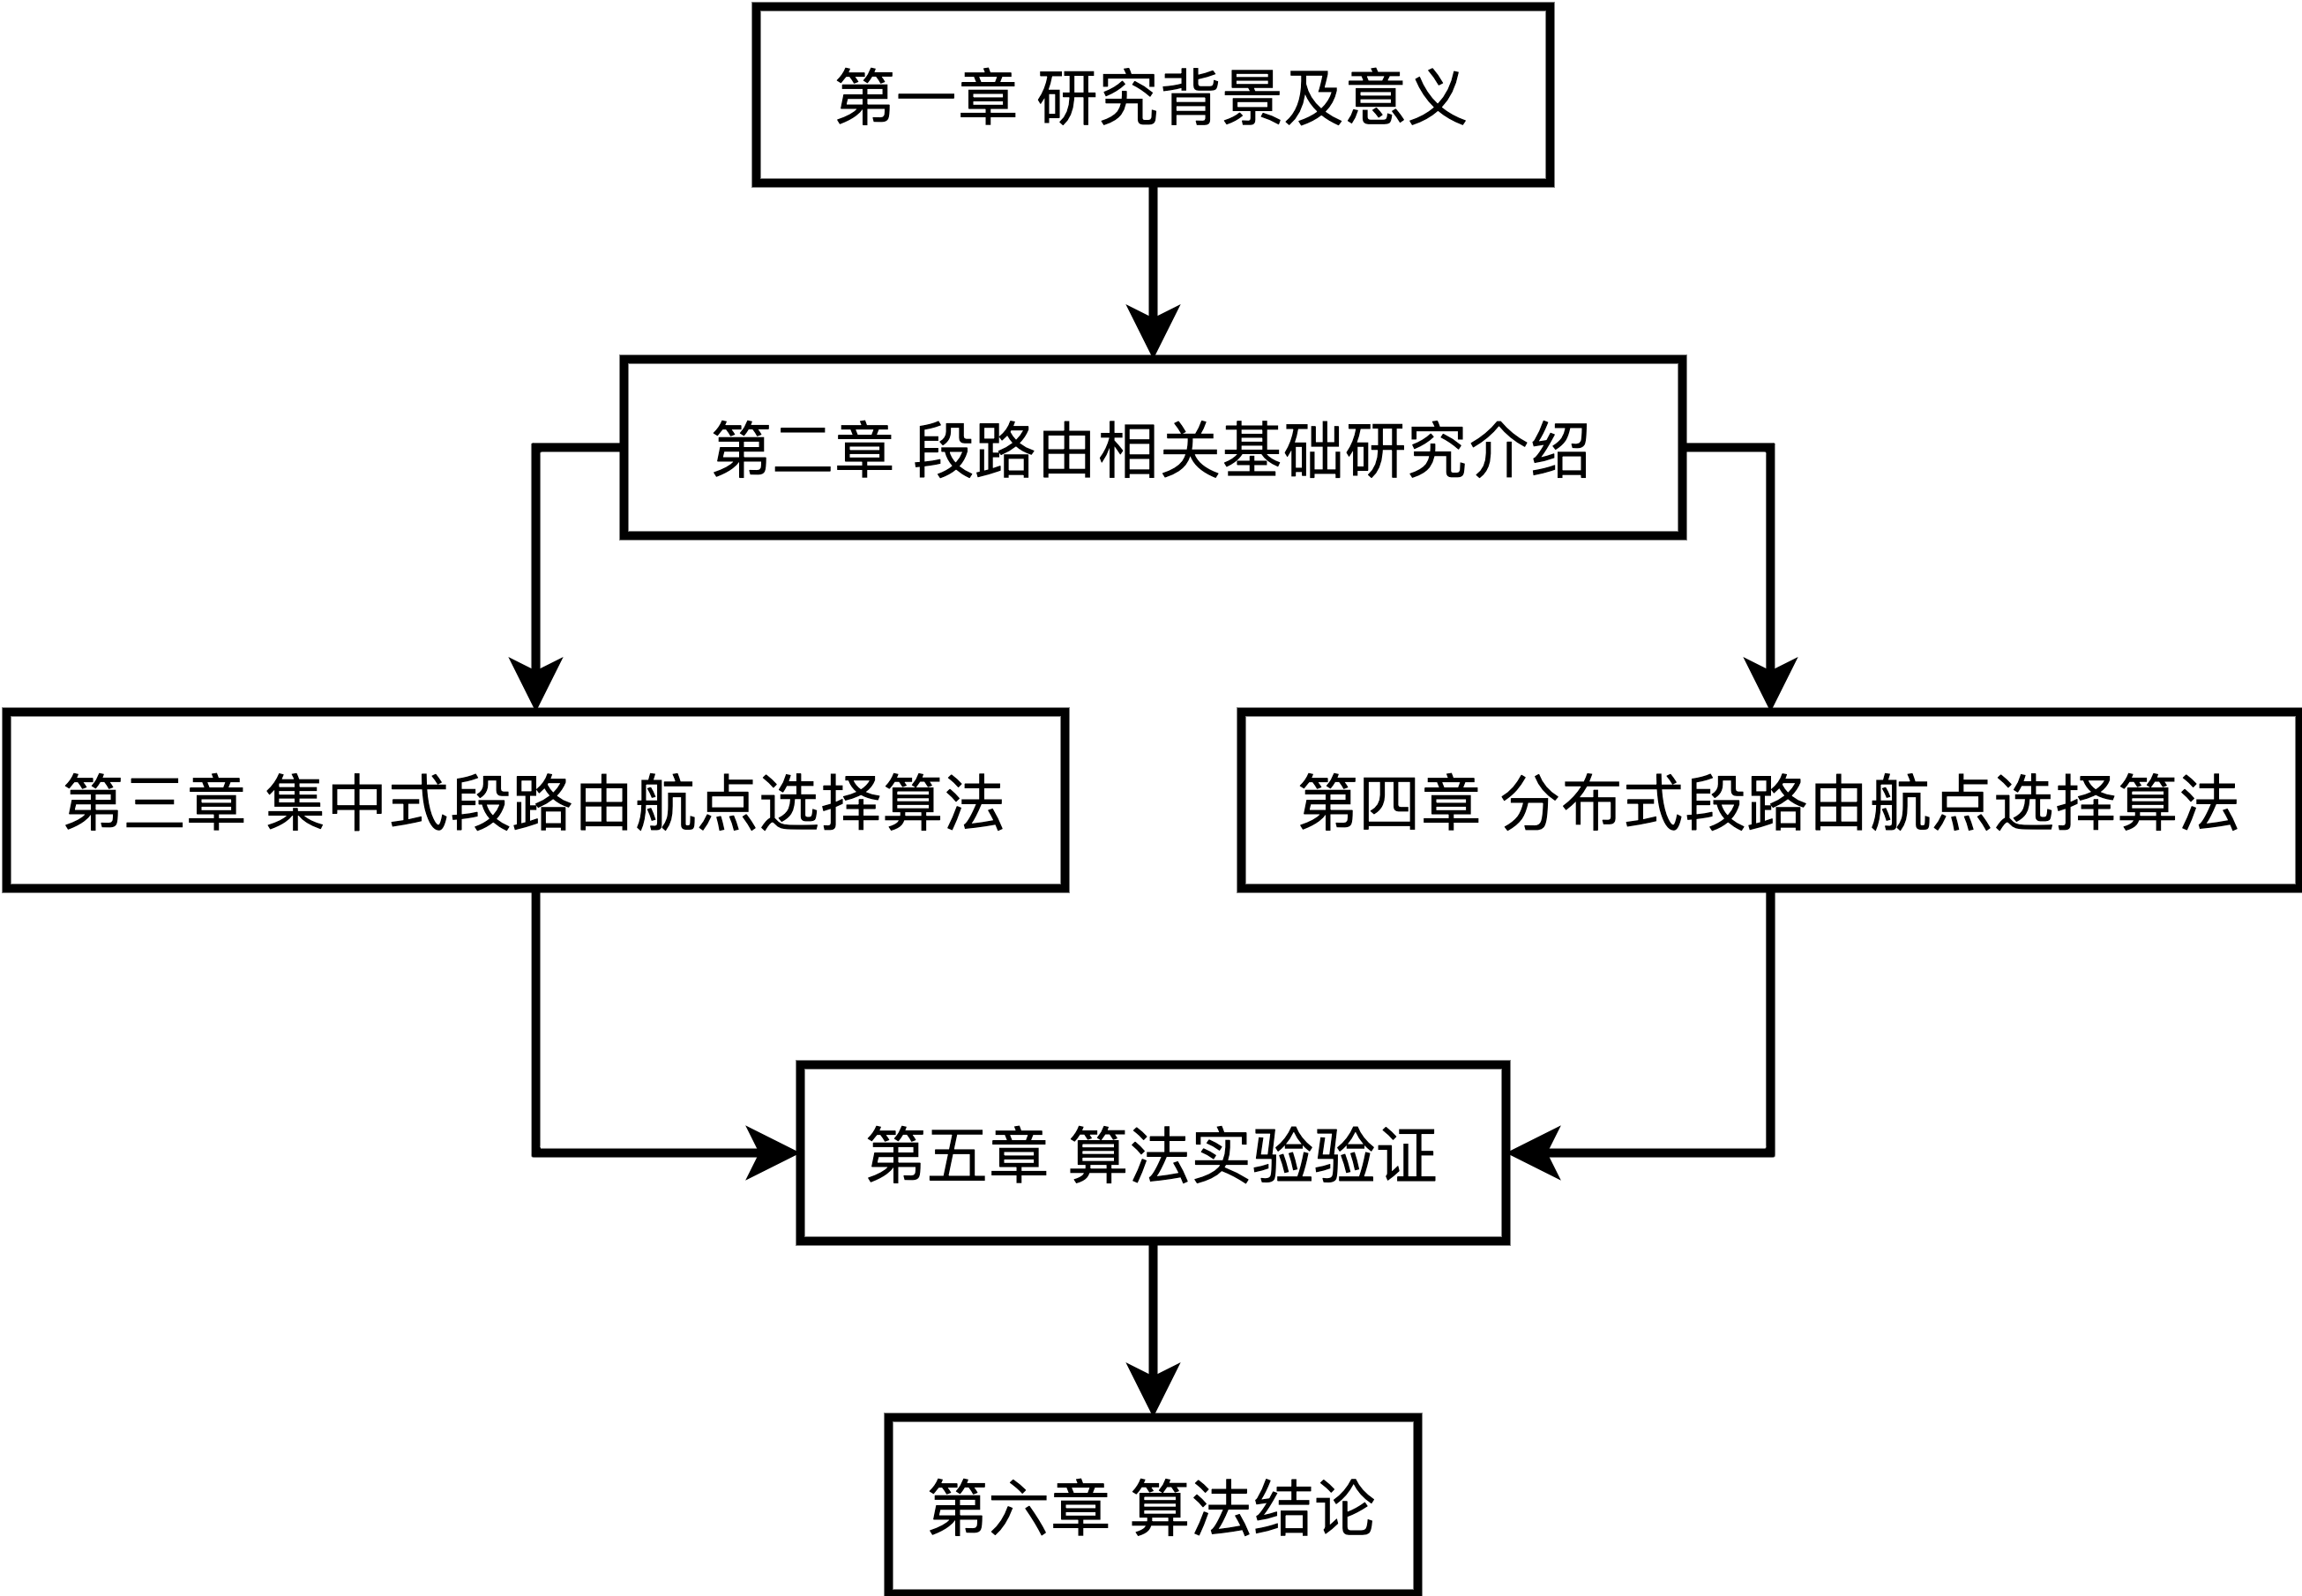
\includegraphics[width=0.95\textwidth]{./figures/ch1-research-relationship.png}}
\caption{各部分研究内容关系图}
\label{fig-ch1-research-relationship}
\end{figure}

首先在第一章对时延研究背景和段路由研究背景和现状进行梳理,阐述保障时延的段路由需要解决的问题和面临的挑战,分析保障时延的段路由的意义和与网络中其他层级技术的相关性,最后给出论文的主要篇章结构安排。

其次在第二章进行相关基础研究的介绍,这将包涵三点,其一是对段路由的一个简单的功能梳理;第二是对时延保障相关的网络技术进行分析,得出对时延保障值得研究的方向总结;第三是对网络中时延信息的获取方案进行梳理,总结使用带内遥测获取时延信息进行控制计算的方案。

然后在第三章将基于集中式软件定义网络控制器全局视角的优点,着重研究了集中式的段路由选择航点的算法,其核心难点在于对网络拓扑的数据规模进行降维,降低算法的时间复杂度。第三章讲对集中式段路由航点列表生成问题进行模型建立、算法目的分析、算法实现以及基于算法时间复杂度分析。

在第四章中将扩大网络的规模,因此会从分布式的角度为段路由选择航点列表,第四章算法的主要优化目的有:降低时延探测流量的比重,降低段路由跳数对网络吞吐量的影响,在合适的范围保障业务流量的端到端时延。第四章参考了部分边界网关协议相关协议的设计细节,将惩罚值和节点聚合引入分布式段路由节点计算的核心数据结构。

在第五章将对第三、第四章提到的两个算法进行实验验证,最终证明在使用集中式控制器进行计算段路由航点列表时将时延因素考虑进来是有益于服务流量时延保障需求的,使用分布式段路由航点生成算法在牺牲一定程度的网络吞吐量情况下对时延保障具有一定效果。

最后在第六章对整个论文的工作做一总结并且计划未来在工作中继续研究的方向。

%% 本章参考文献
\ifx\usechapbib\empty
\nocite{BSTcontrol}
\setcounter{NAT@ctr}{0}
\bibliographystyle{buptgraduatethesis}
\bibliography{bare_thesis}
\fi
